\documentclass[12pt]{article}
\usepackage[margin=1in]{geometry} 
\usepackage{amsmath,amsthm,amssymb,amsfonts,enumerate,listings,graphicx,epstopdf,siunitx}
\graphicspath{~/Documents/school/fall16/stat586/hw2}
 
\newcommand{\N}{\mathbb{N}}
\newcommand{\Z}{\mathbb{Z}}
 
\newenvironment{problem}[2][Problem]{\begin{trivlist}
\item[\hskip \labelsep {\bfseries #1}\hskip \labelsep {\bfseries #2.}]
  \vspace{1 cm}
}{\end{trivlist}}

\begin{document}
\title{Homework Set 2}
\author{Taylor Bodin}
\maketitle

\begin{problem}{3.1}
\item
  \begin{enumerate}[a.]
    \item %A
      Not a valid CDF because $F_X(x)$ decreases.
    \item %B
      This is a valid CDF since it satisfies all the properties of a CDF
    \item %C
      This is a valid CDF since it satisfies all the properties of a CDF
    \item %D
      Not a valid CDF because: $F_x(\infty) \neq 1$
  \end{enumerate}
\end{problem}

\begin{problem}{3.3}
\item
  $F_X(x) = \left(\frac{1}{2} + \frac{1}{\pi}\tan^{-1}(x)\right)u(x)$
  \begin{enumerate}[a.]
    \item %A
      $P(X < 2) = F_X(2) = .8524$
    \item %B
      $P(X>4) = 1-F_X(4) = 1 - (.9220) = \num{7.798e-2}$
    \item %C
      $P(1<x<3) = F_X(3) - F_X(1) = .8976 - .7500 = .1476$
    \item %D
      $P(X>2 | X<4) = \frac{P(X>2 \cap X<4)}{P(X<4)} = \frac{F_X(4)
      -F_X(2)}{F_X(4)} = \num{7.549e-2}$
  \end{enumerate} 
\end{problem}

\begin{problem}{3.5} %TODO: FIGURE A.
\item
  \begin{enumerate}[a.] 
    \item %A. TODO: FIGURE
%     \begin{figure}[htpb]
%       \centering
%       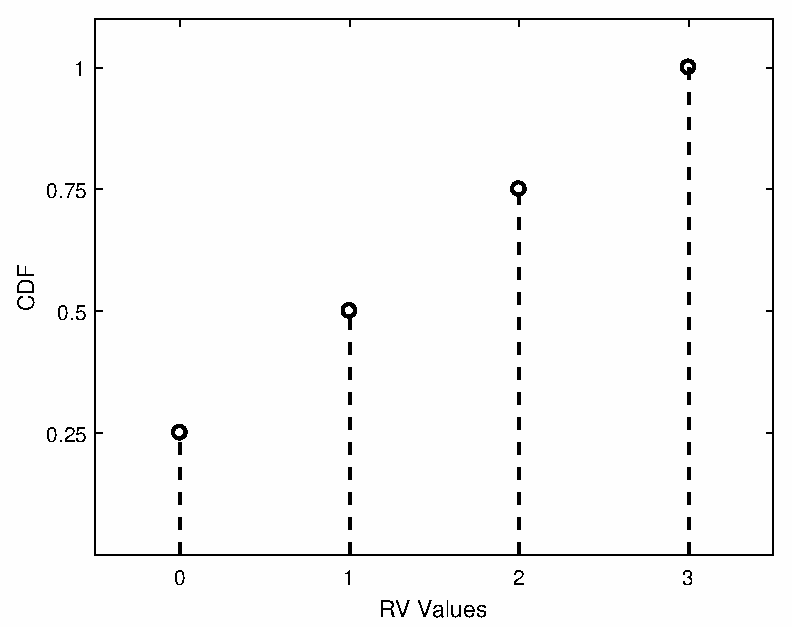
\includegraphics[width=\textwidth,height=\textheight,keepaspectratio]{fig_3_5.eps}
%       \caption{Problem 3.5, Sketch of the CDF of X}
%     \end{figure}
    \item %B.
      $F_X(x) = .25u(x) + .25u(x-1) + .25u(x-2) +.25u(x-3)$
  \end{enumerate}
\end{problem}

\begin{problem}{3.7}
\item
  \begin{enumerate}[a.]
    \item %A.
      Since $a_k$ is basically a PMF, it must satisfy the same conditions. \\
      Specifically, $\sum_{k=0}^\infty a_k = 1$ and $a_k \geq 0 \forall k$.
    \item %B.
      $P(X \leq n) = \sum_{k=0}^n a_k u(x-k)$
  \end{enumerate}
\end{problem}

\begin{problem}{3.9}
\item
  \begin{enumerate}[a.]
    \item %A.
      $P(X = 0) = F_X(0)-F_X(0) = 0, \\ P(X=1) = F_X(1)-F_X(1) = 0$
    \item %B
      $P(X < 0) = F_X(0) = \frac{1}{2}, \\
      P(X>\frac{1}{2}) = 1 - F_X(\frac{1}{2}) = 1-\frac{3}{4} = \frac{1}{4}$
    \item %C.
      $P(X>\frac{1}{2} | X > 0) = \frac{P((X > 0)\cap(X >\frac{1}{2}))}{P(X>0)}
      = \frac{P(X>\frac{1}{2})}{P(X>0)} = \frac{1-F_X(\frac{1}{2})}{1-F_X(0)} 
      = \frac{\frac{1}{4}}{\frac{1}{2}} = \frac{1}{2}$ 
  \end{enumerate}
\end{problem}

\begin{problem}{3.11} %TODO: FIGURES
\item
  \begin{enumerate}[a.]
    \item %A.
      \begin{align*}
        F_X(x) &= \int_{-\infty}^{x} 0dy(1-u(t)) + \int_{0}^{x} dy  \ u(t) \\
        &= 0 + y\big|_{y=0}^x \\
        &=\begin{cases}
            0 & x \leq 0 \\
            x & 0 < x \geq 1 \\
            1 & x > 1
          \end{cases}
      \end{align*}
    \item %TODO A. Figure
%     \begin{figure}[htpb]
%       \centering
%       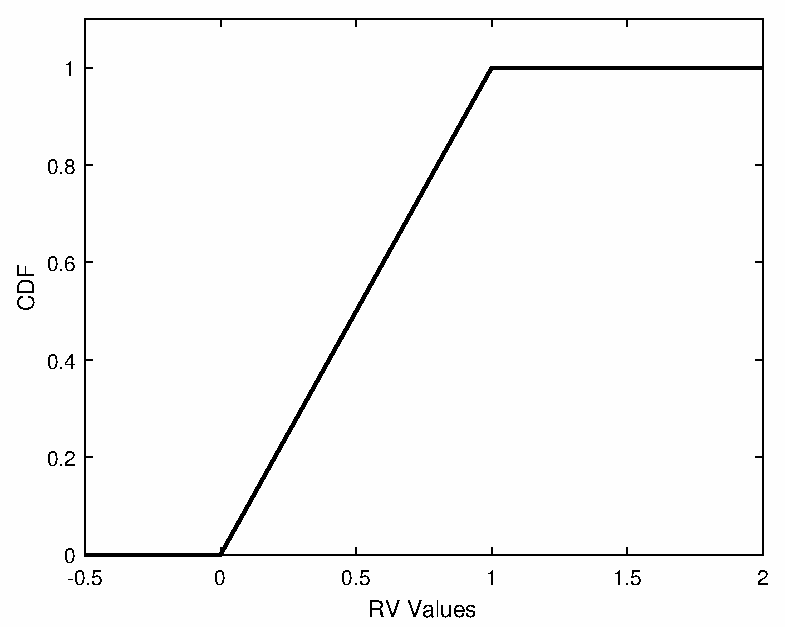
\includegraphics[width=\textwidth,height=\textheight,keepaspectratio]{fig_3_11_a.eps}
%       \caption{Problem 3.11 A, Sketch of the CDF of X}
%     \end{figure}
    \item %TODO B.
      \begin{align*}
        F_X(x) &= \int_{-\infty}^{x} 0 \ dy = 0 \\
          &+ \int_{0}^{x} y  dy \ (u(t)-u(t-1))) \\
          &+ \int_0^1 y  dy + \int_1^x (2-y)dy \ (u(t-2) - u(t-2)) \\
        &=\begin{cases}
            0 & x \leq 0 \\
            \frac{x^2}{2} & 0 < x \geq 1 \\
            -\frac{x^2}{2} + 2x - 1 & 1 > x \geq 2 \\
            1 & x > 2
          \end{cases}
      \end{align*}
    \item %TODO B. Figure
%     \begin{figure}[htpb]
%       \centering
%       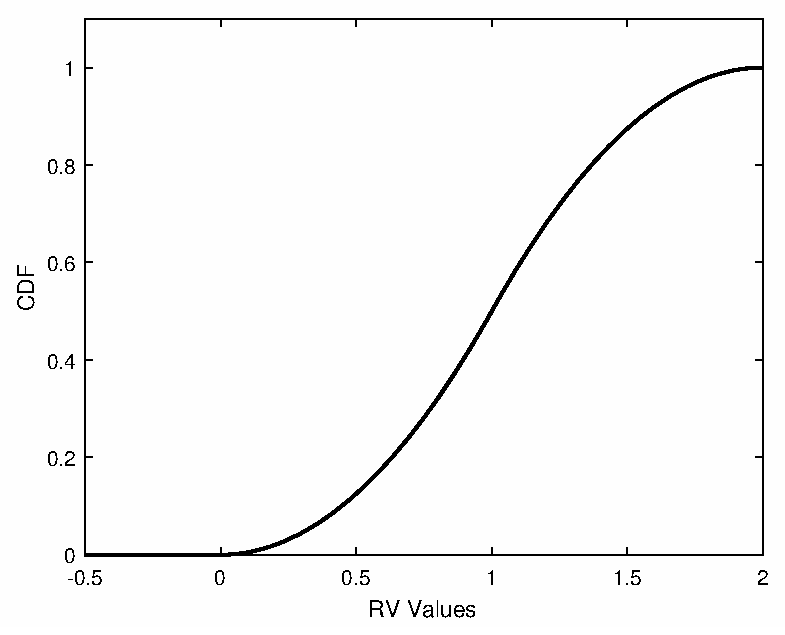
\includegraphics[width=\textwidth,height=\textheight,keepaspectratio]{fig_3_11_b.eps}
%       \caption{Problem 3.11 B, Sketch of the CDF of X}
%     \end{figure}
  \end{enumerate}
\end{problem}

\begin{problem}{3.13}
\item
  \begin{enumerate}[a.]
    \item %A. 
      $f_X(x)$ is of the form of a exponential random variable. Therefore,
      c is known to be equal to the coefficient of the exponent multiplied
      by negative 1. Thus, $c = 2$. The CDF is also known to be 
      $F_X(x) = \left[1 - e^{-\frac{x}{b}}\right]u(x)$ and is used for the 
      following problems. 
    \item %B.
      $P(X>2) = 1 - F_X(2) = 1 - .8647 = .1353$
    \item %C.
      $P(X<3) = F_X(3) = .9975$
    \item %D.
      $P(X < 3|X>2) = \frac{P(X<3)\cap P(X>2)}{P(X>2)}
      = \frac{F_X(3) - F_X(2)}{F_X(2)} = \num{1.613e-2}$
  \end{enumerate}
\end{problem}

\begin{problem}{3.15}
\item
  \begin{enumerate}[a.]
    \item %A.
    Solving the equation $1 = \int_{-5}^5 \frac{c}{\sqrt{25-x^2}}dx$ for c
      yields $c = \frac{1}{\pi}$. \\
      Substituting c back into the PDF and integrating from -5 to x produces
      the CDF: $F_X(X) = \frac{2\sin^{-1}(\frac{x}{5})+\pi}{2\pi}$
    \item %B.
      $P(X>2) = 1 - F_X(2) = 1 - .6310 = .3690$
    \item %C.
      $P(X<3) = F_X(3) = .7048$
    \item %D.
      $P(X < 3|X>2) = \frac{P(X<3)\cap P(X>2)}{P(X>2)}
      = \frac{F_X(3) - F_X(2)}{F_X(2)} = .1170$
  \end{enumerate}
\end{problem}

\begin{problem}{3.17}
\item
  \begin{enumerate}[a.]
    \item %A.
      $f_x \geq 0 \ \forall \ x$ and $\int_{-\infty}^{\infty} f_x(x)dx = 1$.
      Therefore, $f_x$ is a valid PDF.
    \item %B.
      $f_x \geq 0 \ \forall \ x$ but $\int_{-\infty}^{\infty} f_x(x)dx \approx 1.333$.
      Therefore, $f_x$ is not a valid PDF.
    \item %C.
      $f_x \geq 0 \ \forall \ x$ but $\int_{-\infty}^{\infty} f_x(x)dx =
      \frac{1}{4}$. Therefore, $f_x$ is not a valid PDF.
    \item %D.
      $f_x \ngeq 0 \ \forall \ x$ and $\int_{-\infty}^{\infty} f_x(x)dx = 0$.
      Therefore, $f_x$ is not a valid PDF.
  \end{enumerate}
\end{problem}

\begin{problem}{3.19}
\item %A.
  \begin{align*}
    I &= \int_{-\infty}^{\infty} e^{-\frac{x^2}{2}}dx = \sqrt{2\pi} \\
    I^2 &= \left(\int_{-\infty}^{\infty} e^{-\frac{x^2}{2}}dx \right)
    \left( \int_{-\infty}^{\infty} e^{-\frac{y^2}{2}}dy \right) = 2\pi \\
    &= \int_{-\infty}^{\infty} \int_{-\infty}^{\infty} e^{-\frac{x^2+y^2}{2}}dydx
    & & \textrm{Transform to polar coordinates} \\
    &= \int_{0}^{2\pi} \int_{0}^{\rho} e^{-\frac{\rho^2}{2}}\rho d\rho d\theta \\
    &= \int_{0}^{2\pi} \int_{a}^{b} -e^{u}du d\theta & & u = -\frac{\rho^2}{2} \\
    &= \int_{0}^{2\pi} -e^{-\frac{\rho}{2}} \big|_{\rho = 0}^{\infty} d\theta \\
    &= \int_{0}^{2\pi} d\theta \\
    &= 2\pi
  \end{align*}
\end{problem}

\begin{problem}{3.21} %TODO: Analytical Solution to A, and B
\item
  \begin{enumerate}[a.]
    \item %A. TODO: Analytical Solution?
      Using WolframAlpha\textsuperscript{\textregistered}, the value of c was found to be 
      $\frac{\sqrt{\frac{2}{\pi}}}{\sqrt[8]{e}} \approx .7041$
    \item %B. TODO calculate m
      The equation $c = \frac{\sqrt{\frac{2}{\pi}}}{\sqrt[8]{e}}$ was solved to 
      find that $c \approx .5667$ \\ 
      To find m, the exponent was factored to
  \end{enumerate}
\end{problem}

\begin{problem}{3.23} %TODO
\item
\end{problem}
\end{document}

\begin{problem}{3.25} %TODO
\item
\end{problem}

\begin{problem}{3.27} %TODO
\item
\end{problem}

\begin{problem}{3.29} %TODO
\item
\end{problem}

\begin{problem}{3.31} %TODO
\item
\end{problem}

\begin{problem}{3.33} %TODO
\item
\end{problem}


\end{document}
